\documentclass[a4paper,12pt]{article}
\usepackage[a4paper,top=1.3cm,bottom=2cm,left=1.5cm,right=1.5cm,marginparwidth=0.75cm]{geometry}
\usepackage{cmap}
\usepackage{mathtext}
\usepackage[T2A]{fontenc}
\usepackage[utf8]{inputenc}
\usepackage[english,russian]{babel}
\usepackage{siunitx}
\usepackage{enumitem}
\usepackage{placeins}

\usepackage{graphicx}

\usepackage{wrapfig}
\usepackage{tabularx}
\usepackage{multirow}

\usepackage{hyperref}
\usepackage[rgb]{xcolor}
\hypersetup{
colorlinks=true,urlcolor=blue
}
\usepackage{amsmath,amsfonts,amssymb,amsthm,mathtools}
\usepackage{icomma}
\mathtoolsset{showonlyrefs=false}
\usepackage{euscript}
\usepackage{mathrsfs}
\DeclareMathOperator{\sgn}{\mathop{sgn}}
\newcommand*{\hm}[1]{#1\nobreak\discretionary{}
{\hbox{$\mathsurround=0pt #1$}}{}}

%%% Заголовок
\author{Макаров Лев Евгеньевич}
\title{Лабораторная работа №3.5.1

Изучение плазмы газового разряда в неоне
}
\date{\today}

\begin{document}

\begin{titlepage}
	\begin{center}
		{\large МОСКОВСКИЙ ФИЗИКО-ТЕХНИЧЕСКИЙ ИНСТИТУТ (НАЦИОНАЛЬНЫЙ ИССЛЕДОВАТЕЛЬСКИЙ УНИВЕРСИТЕТ)}
	\end{center}
	\begin{center}
		{\large Физтех-школа фотоники, электроники и молекулярной физики}
	\end{center}
	
	
	\vspace{4.5cm}
	{\huge
		\begin{center}
			{\bf Отчёт о выполнении лабораторной работы 4.4.1}\\
			Амплитудная дифракционная решетка
		\end{center}
	}
	\vspace{2cm}
	\begin{flushright}
		{\LARGE Автор:\\ Макаров Лев Евгеньевич \\
			\vspace{0.2cm}
			Б04-306}
	\end{flushright}
	\vspace{8cm}
	\begin{center}
		Долгопрудный 2025
	\end{center}
\end{titlepage}

\section{Введение}

\textbf{Цель работы:} 
\begin{enumerate}
	\item Знакомство с работой и настройкой гониометра Г5
    \item Определение спектральных характеристик амплитудной решётки
\end{enumerate}

\textbf{В работе используются:} 
\begin{itemize}
    \item гониометр
    \item ртутная лампа
    \item амплитудная решетка
    \item призменный уголковый отражатель
    \item щель с микрометрическим винтом
\end{itemize}
\medskip

\section{Теоретические сведения}

\subsection*{Амплитудная дифракционная решётка}

Амплитудная решётка состоит из непрозрачного экрана с большим числом $N$ параллельных щелей (штрихов) с периодом $d$ и шириной штриха $b$.

\FloatBarrier
\begin{figure}[h]
    \centering
    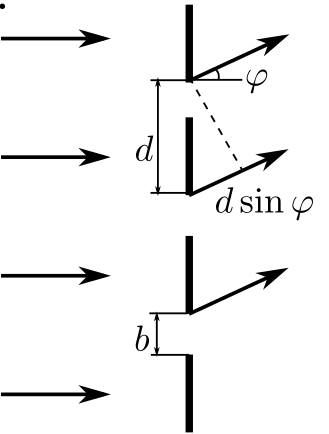
\includegraphics[width=0.3\textwidth]{difraction.png}
    \caption{Схема дифракции на амплитудной решётке}
    \label{pic:difraction}
\end{figure}
\FloatBarrier

Интенсивность света максимальна для углов $\varphi_m$, удовлетворяющих уравнению:
\begin{equation}
    d \sin \varphi_m = m \lambda,
\end{equation}
где $m = 0, \pm 1, \pm 2, \dots$ — порядок спектра.

Интенсивность распределяется согласно закону Фраунгофера:
\begin{equation}
    dW = I_0 \frac{b^2}{\lambda} \left[\frac{\sin(\pi b \sin \varphi / \lambda)}{\pi b \sin \varphi / \lambda}\right]^2 \left[\frac{\sin(\pi N d \sin \varphi / \lambda)}{\sin(\pi d \sin \varphi / \lambda)}\right]^2 d\varphi.
\end{equation}

\section{Экспериментальная установка}

\subsection*{Устройство гониометра Г5}

Гониометр Г5 состоит из неподвижного коллиматора, вращающегося столика для исследуемых объектов и алидады с закрепленной зрительной трубой.

\FloatBarrier
\begin{figure}[h]
    \centering
    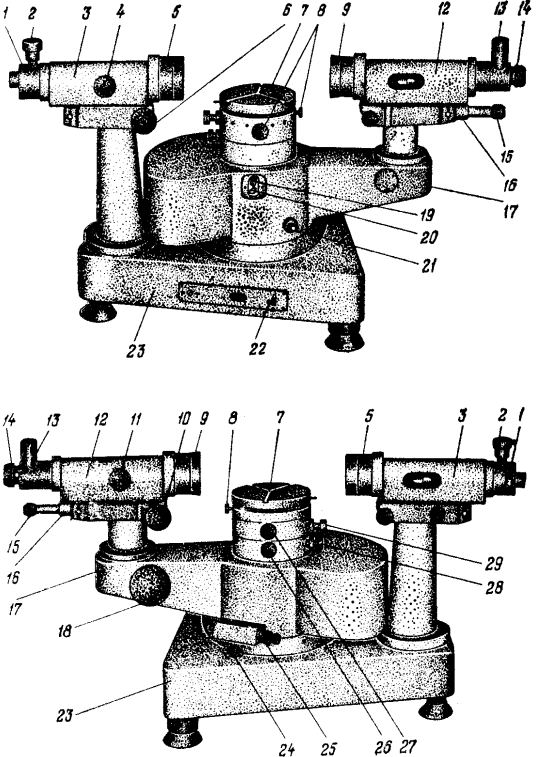
\includegraphics[width=0.5\textwidth]{goniometer.png}
    \caption{Внешний вид гониометра Г5}
    \label{pic:goniometer}
\end{figure}
\FloatBarrier

Коллиматор позволяет формировать параллельный пучок света, который направляется на исследуемый объект. Регулировка ширины и высоты коллиматорной щели осуществляется с помощью микрометрического винта и диафрагмы. Юстировка коллиматора производится специальными винтами.

Автоколлимационное устройство позволяет точнее настраивать гониометр. Оно состоит из зрительной трубы с объективом и окуляром с перекрестием.

\FloatBarrier
\begin{figure}[h]
    \centering
    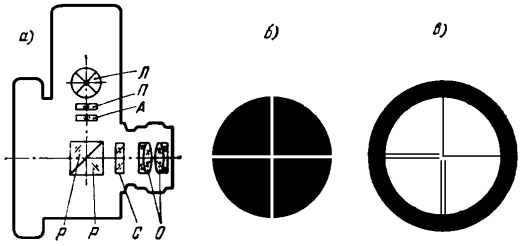
\includegraphics[width=0.4\textwidth]{autocollimat.png}
    \caption{Автоколлимационное устройство}
    \label{pic:autocollimat}
\end{figure}
\FloatBarrier

Юстировка гониометра включает проверку параллельности оптических осей компонентов и корректировку установки исследуемого объекта. Измерение углов осуществляется путем вращения алидады с отсчетом по шкале.

\subsection*{Спектр ртутной лампы}

Каждая линия спектра имеет свою ширину и тонкую структуру. Ниже приведены некоторые интегральные характеристики спектральных линий для лампы ДРШ-250.

\begin{figure}[h]
    \centering
    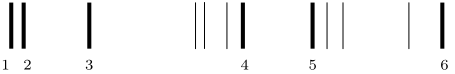
\includegraphics[width=0.6\textwidth]{lamp_spectr.png}
    \caption{Спектр ртутной лампы ДРШ-250}
    \label{pic:lamp_spectr}
\end{figure}

\begin{table}[h]
    \centering
    \caption{Характеристики спектра ртутной лампы ДРШ-250}
    \begin{tabular}{|c|c|c|c|c|c|c|}
        \hline
        № & 1 & 2 & 3 & 4 & 5 & 6 \\ \hline
        $\lambda$ (нм) & 579.1 & 577.0 & 546.1 & 491.6 & 435.8 & 404.7 \\ \hline
        Цвет & Жёлтый & Жёлтый & Зелёный & Голубой & Синий & Фиолетовый \\ \hline
        Яркость & 10 & 8 & 10 & 4 & 4 & 3 \\ \hline
    \end{tabular}
    \label{tab:mercury_spectrum}
\end{table}

\section{Результаты измерений и обработка данных}

\subsection*{I. Настройка гониометра}

Проведем юстировку гониометра и установим начало отсчета.

\subsection*{II. установка решетки}

\begin{enumerate}
    \item Настроим зрительную трубу на изображение щели коллиматора так, чтобы видимый размер её изображения был менее половины поля зрения. Начальный угол отсчета $180^\circ$. Повернем зрительную трубу на $90^\circ$.
    \item Поставим эшелет на столик рабочей поверхностью к коллиматору. Вращая верхнюю часть столика найдем ахроматическое изображение щели. Тогда угол падения света на эшелет равен $\psi = 180^\circ$.
    \item Винтом 8 (перпендикулярным плоскости эшелета) совмести центр изображения щели с горизонтальным штрихом отсчетного винта. Отведем алидаду в стороны и вторым винтом 8 устраним вертикальное расхождение.
\end{enumerate}

\subsection*{III. Исследование спектра ртутной лампы}

\begin{enumerate}[resume]
    \item Подберем ширину входной щели так, чтобы были видны желтые линии ртутного спектра. Установим высоту щели $\sim$2 мм.
    \item Измерим угловые координаты спектральных линий ртути в рабочем порядке. Результаты измерений запишем в таблицу \ref{table:1}.
\end{enumerate}

\FloatBarrier
\begin{table}[!ht]
    \centering
    \caption{\textit{Измерение угловых координат спектральных линий}}
    \begin{tabular}{|l|l|l|l|}
        \hline
                       & град & мин & сек \\ \hline
        правая фиол    & 292  & 31  & 0   \\ \hline
        левая фиол     & 292  & 56  & 0   \\ \hline
        самая тусклая  & 293  & 52  & 0   \\ \hline
        средняя яркая  & 293  & 54  & 0   \\ \hline
        самая яркая    & 293  & 57  & 0   \\ \hline
        голубая        & 296  & 14  & 50  \\ \hline
        зеленая        & 298  & 16  & 55  \\ \hline
        желтая правая  & 299  & 25  & 32  \\ \hline
        желтая левая    & 299  & 30  & 27  \\ \hline
        красная правая & 300  & 30  & 20  \\ \hline
        красная левая  & 300  & 42  & 59  \\ \hline
    \end{tabular}
    \label{table:1}
\end{table}
\FloatBarrier

Дальнейшие пункты работы не выполнялись

\subsection*{Обработка результатов}

\begin{enumerate}
    \item Для угла падения $\psi = 45^\circ$ построим график зависимости $(\sin{\phi_m} - \sin{\psi})$ от длины волны. График изобразим на рис. \ref{graph:1}.
\end{enumerate}

\FloatBarrier
\begin{figure}[!ht]
        \centering
	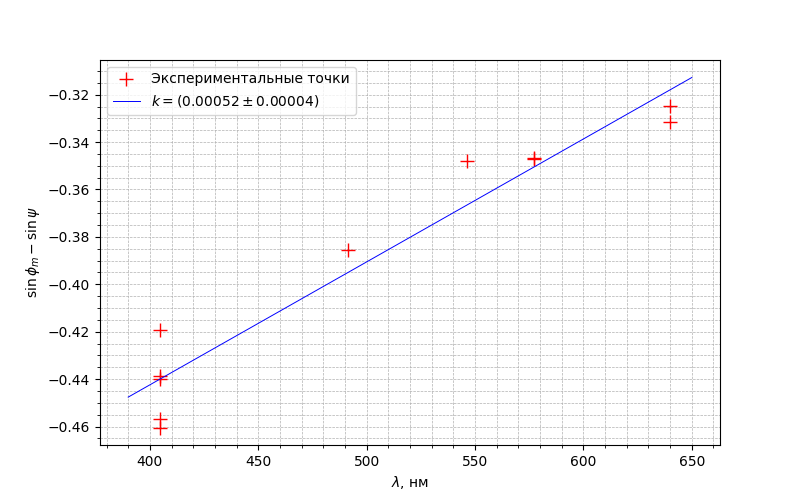
\includegraphics[width=1.0\textwidth]{graph-1.png}
	\caption{\textit{Зависимость $(\sin{\phi_m} - \sin{\psi})$ от $\lambda$}}
	\label{graph:1}
\end{figure}
\FloatBarrier

Из соотношения следует

\begin{equation*}
    d (\sin{\phi_m} - \sin{\psi}) = \lambda m \implies k = \frac{m}{d} \implies d = \frac{m}{k} \approx (1930 \pm 10) \ \text{нм}
\end{equation*}





\end{document}
